%% GENERATED by make_result_figs.py from results/T1v3_heldout.csv, rbrl_ppo5_v3_<c>.csv, T21v3_<c>.csv, T21v3_pers_<c>.csv, T17v3_<c>.csv; do not edit
\begin{figure}[t]
\centering
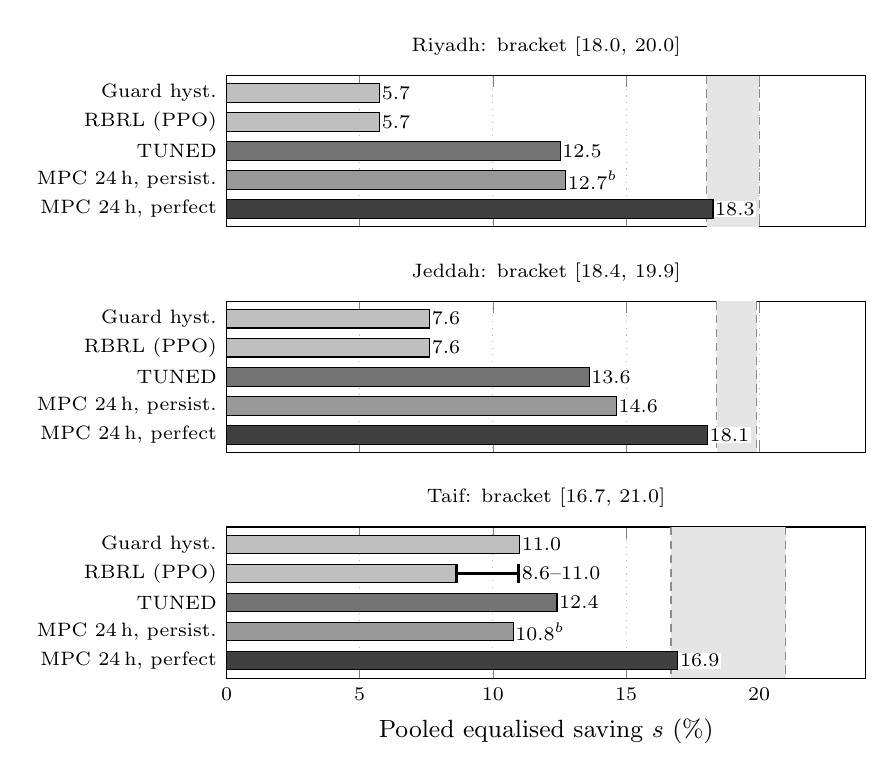
\begin{tikzpicture}
\begin{axis}[
  name=p0, width=0.80\columnwidth, height=3.5cm, scale only axis=false,
  xmin=0, xmax=24, ymin=0.4, ymax=5.6, y dir=reverse,
  ytick={1,2,3,4,5}, yticklabels={{Guard hyst.},{RBRL (PPO)},{TUNED},{MPC $24\,$h, persist.},{MPC $24\,$h, perfect}},
  y tick style={draw=none}, xtick={0,5,10,15,20},
  xticklabels={},
  xmajorgrids, grid style={dotted,gray!50},
  tick label style={font=\scriptsize}, label style={font=\small},
  title={Riyadh: bracket $[18.0,\,20.0]$},
  title style={font=\scriptsize, yshift=-0.6ex},
]
\fill[black!10] (axis cs:18.0228,0.4) rectangle (axis cs:20.0,5.6);
\draw[black!45, densely dashed] (axis cs:18.0228,0.4) -- (axis cs:18.0228,5.6);
\draw[black!45, densely dashed] (axis cs:20.0,0.4) -- (axis cs:20.0,5.6);
\fill[black!25, draw=black, thin] (axis cs:0,0.6799999999999999) rectangle (axis cs:5.7452,1.32);
\node[font=\scriptsize, anchor=west, inner sep=0.6pt, fill=white] at (axis cs:5.7452,1) {5.7};
\fill[black!25, draw=black, thin] (axis cs:0,1.68) rectangle (axis cs:5.7446,2.32);
\node[font=\scriptsize, anchor=west, inner sep=0.6pt, fill=white] at (axis cs:5.7452,2) {5.7};
\fill[black!55, draw=black, thin] (axis cs:0,2.68) rectangle (axis cs:12.5260,3.32);
\node[font=\scriptsize, anchor=west, inner sep=0.6pt, fill=white] at (axis cs:12.5260,3) {12.5};
\fill[black!40, draw=black, thin] (axis cs:0,3.68) rectangle (axis cs:12.7357,4.32);
\node[font=\scriptsize, anchor=west, inner sep=0.6pt, fill=white] at (axis cs:12.7357,4) {12.7$^{b}$};
\fill[black!75, draw=black, thin] (axis cs:0,4.68) rectangle (axis cs:18.2638,5.32);
\node[font=\scriptsize, anchor=west, inner sep=0.6pt, fill=white] at (axis cs:18.2638,5) {18.3};
\end{axis}
\begin{axis}[
  at={(p0.below south west)}, anchor=above north west, yshift=-1mm,
  name=p1, width=0.80\columnwidth, height=3.5cm, scale only axis=false,
  xmin=0, xmax=24, ymin=0.4, ymax=5.6, y dir=reverse,
  ytick={1,2,3,4,5}, yticklabels={{Guard hyst.},{RBRL (PPO)},{TUNED},{MPC $24\,$h, persist.},{MPC $24\,$h, perfect}},
  y tick style={draw=none}, xtick={0,5,10,15,20},
  xticklabels={},
  xmajorgrids, grid style={dotted,gray!50},
  tick label style={font=\scriptsize}, label style={font=\small},
  title={Jeddah: bracket $[18.4,\,19.9]$},
  title style={font=\scriptsize, yshift=-0.6ex},
]
\fill[black!10] (axis cs:18.4099,0.4) rectangle (axis cs:19.9,5.6);
\draw[black!45, densely dashed] (axis cs:18.4099,0.4) -- (axis cs:18.4099,5.6);
\draw[black!45, densely dashed] (axis cs:19.9,0.4) -- (axis cs:19.9,5.6);
\fill[black!25, draw=black, thin] (axis cs:0,0.6799999999999999) rectangle (axis cs:7.6244,1.32);
\node[font=\scriptsize, anchor=west, inner sep=0.6pt, fill=white] at (axis cs:7.6244,1) {7.6};
\fill[black!25, draw=black, thin] (axis cs:0,1.68) rectangle (axis cs:7.6244,2.32);
\node[font=\scriptsize, anchor=west, inner sep=0.6pt, fill=white] at (axis cs:7.6279,2) {7.6};
\fill[black!55, draw=black, thin] (axis cs:0,2.68) rectangle (axis cs:13.6163,3.32);
\node[font=\scriptsize, anchor=west, inner sep=0.6pt, fill=white] at (axis cs:13.6163,3) {13.6};
\fill[black!40, draw=black, thin] (axis cs:0,3.68) rectangle (axis cs:14.6377,4.32);
\node[font=\scriptsize, anchor=west, inner sep=0.6pt, fill=white] at (axis cs:14.6377,4) {14.6};
\fill[black!75, draw=black, thin] (axis cs:0,4.68) rectangle (axis cs:18.0577,5.32);
\node[font=\scriptsize, anchor=west, inner sep=0.6pt, fill=white] at (axis cs:18.0577,5) {18.1};
\end{axis}
\begin{axis}[
  at={(p1.below south west)}, anchor=above north west, yshift=-1mm,
  name=p2, width=0.80\columnwidth, height=3.5cm, scale only axis=false,
  xmin=0, xmax=24, ymin=0.4, ymax=5.6, y dir=reverse,
  ytick={1,2,3,4,5}, yticklabels={{Guard hyst.},{RBRL (PPO)},{TUNED},{MPC $24\,$h, persist.},{MPC $24\,$h, perfect}},
  y tick style={draw=none}, xtick={0,5,10,15,20},
  xlabel={Pooled equalised saving $s$ (\%)},
  xmajorgrids, grid style={dotted,gray!50},
  tick label style={font=\scriptsize}, label style={font=\small},
  title={Taif: bracket $[16.7,\,21.0]$},
  title style={font=\scriptsize, yshift=-0.6ex},
]
\fill[black!10] (axis cs:16.6880,0.4) rectangle (axis cs:21.0,5.6);
\draw[black!45, densely dashed] (axis cs:16.6880,0.4) -- (axis cs:16.6880,5.6);
\draw[black!45, densely dashed] (axis cs:21.0,0.4) -- (axis cs:21.0,5.6);
\fill[black!25, draw=black, thin] (axis cs:0,0.6799999999999999) rectangle (axis cs:11.0020,1.32);
\node[font=\scriptsize, anchor=west, inner sep=0.6pt, fill=white] at (axis cs:11.0020,1) {11.0};
\fill[black!25, draw=black, thin] (axis cs:0,1.68) rectangle (axis cs:8.6085,2.32);
\draw[black, thick, |-|] (axis cs:8.6085,2) -- (axis cs:11.0020,2);
\node[font=\scriptsize, anchor=west, inner sep=0.6pt, fill=white] at (axis cs:11.0020,2) {8.6--11.0};
\fill[black!55, draw=black, thin] (axis cs:0,2.68) rectangle (axis cs:12.4072,3.32);
\node[font=\scriptsize, anchor=west, inner sep=0.6pt, fill=white] at (axis cs:12.4072,3) {12.4};
\fill[black!40, draw=black, thin] (axis cs:0,3.68) rectangle (axis cs:10.7608,4.32);
\node[font=\scriptsize, anchor=west, inner sep=0.6pt, fill=white] at (axis cs:10.7608,4) {10.8$^{b}$};
\fill[black!75, draw=black, thin] (axis cs:0,4.68) rectangle (axis cs:16.9432,5.32);
\node[font=\scriptsize, anchor=west, inner sep=0.6pt, fill=white] at (axis cs:16.9432,5) {16.9};
\end{axis}
\end{tikzpicture}
\caption{Savings ladder: pooled equalised saving $s$ of five arms in each city, with the clairvoyant bracket $[\mathrm{CLV\ raw},\,B^\ast]$ shaded and its ends dashed (values of Table~\ref{tab:main}; $B^\ast$ under $V_N$, Section~\ref{subsec:bound}). Guard hyst.: the guard hysteresis; RBRL: rule-constrained PPO, the five seeds' range drawn as an interval where it exceeds the rounding. $^{b}$fitted at the pooled $0.10\,$K fallback. The $24\,$h MPC's pooled margin over TUNED, $4.4$ to $5.7$ points with a perfect forecast, becomes $-1.6$ to $1.0$ with a persistence forecast (not resolved); RBRL stays at the level of the guard hysteresis in Riyadh and Jeddah, and in Taif its seeds reach down to $8.6\%$ against the guard's $11.0\%$, a difference under $3$ points that is not resolved.}
\label{fig:ladder}
\end{figure}
